% 原書166--184頁（PDF188--206）、第6章導入および6.1--6.4。
\sectionlink{ツリーレベルの振幅}\label{ch:6}

弦の相互作用を研究する準備が整った。本章では、正の Euler 数を持つ曲面から生じる最低次の振幅を考える。まず、関係する Riemann 面を記述し、必要となる CFT の期待値を計算する。次に散乱振幅を、最初は開弦について、続いて閉弦について調べる。その途中で、開弦理論の重要な一般化である Chan--Paton 因子を導入する。節の最後では CFT に戻り、期待値の一般的な性質をいくつか議論する。

\subsectionlink{Riemann 面}\label{sec:6.1}

正の Euler 数を持つ Riemann 面は、球面、円板、射影平面の三つである。

\subsubsectionlink*{球面}

球面 $S_2$ は、図\ref{fig:6.1} のように二つの座標近傍で覆うことができる。$\rho>1$ として円板 $|z|<\rho$ と $|u|<\rho$ を取り、
\begin{equation}
u=1/z
\tag{6.1.1}\label{eq:6.1.1}
\end{equation}
を満たす点を同一視して貼り合わせる。実際には $\rho\to\infty$ としてもよい。このとき座標 $z$ は「北極」$u=0$ を除くすべての場所で有効である。北極での振る舞いが正則であることを確認する場合を除けば、主に $z$ 座標近傍で計算できる。

両方の座標近傍で平坦な計量を取り、それらを共形変換（座標変換と Weyl 変換）で結ぶことにより、球面を Riemann 面と考えることができる。あるいは、大域的に定義された計量を備えた Riemann 多様体と考えてもよい。一般的な共形ゲージの計量は
\begin{equation}
ds^2=\exp(2\omega(z,\bar z))\,dz\,d\bar z
\tag{6.1.2}\label{eq:6.1.2}
\end{equation}
である。

\begin{figure}[htbp]
\centering
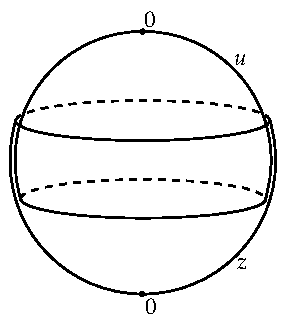
\includegraphics[width=0.65\linewidth]{figures/fig_6_1.pdf}
\caption{$z$ および $u$ 座標近傍から構成した球面。}\label{fig:6.1}
\end{figure}

$dz\,d\bar z=|z|^4du\,d\bar u$ なので、計量が $u=0$ で特異でないための条件は、$z\to\infty$ で $\exp(2\omega(z,\bar z))$ が $|z|^{-4}$ として減衰することである。たとえば、
\begin{equation}
ds^2=\frac{4r^2dz\,d\bar z}{(1+z\bar z)^2}
=\frac{4r^2du\,d\bar u}{(1+u\bar u)^2}
\tag{6.1.3}\label{eq:6.1.3}
\end{equation}
は、半径 $r$、曲率 $R=2/r^2$ の球面を表す。

第5.2節の一般的な議論によれば、球面にはモジュライがなく、六つの CKV がある。したがって特に、すべての計量は、丸い球面の計量 \hyperref[eq:6.1.3]{(6.1.3)} と $(\mathrm{diff}\times\mathrm{Weyl})$ 同値である。これを無限小のレベルで見てみよう。式 \hyperref[eq:5.2.8a]{(5.2.8)} と同様に、正則なテンソル場 $\delta g_{zz}(z)$ と正則なベクトル場 $\delta z(z)$ を探す。これらは球面全体で定義されていなければならないので、$u$ 座標近傍への変換を考える必要がある：
\begin{align}
\delta u&=\frac{\partial u}{\partial z}\delta z=-z^{-2}\delta z,
\tag{6.1.4a}\label{eq:6.1.4a}\\
\delta g_{uu}&=\left(\frac{\partial u}{\partial z}\right)^{-2}\delta g_{zz}=z^4\delta g_{zz}.
\tag{6.1.4b}\label{eq:6.1.4b}
\end{align}
正則な2次微分形式 $\delta g_{zz}$ は、$z$ に関して正則でありながら、無限遠で $z^{-4}$ として消えなければならないので、恒等的にゼロである。一方、CKV $\delta z$ は、$z\to\infty$ で $z^2$ より速く増大しなければ、$u=0$ で正則である。したがって一般的な CKV は
\begin{align}
\delta z&=a_0+a_1z+a_2z^2,
\tag{6.1.5a}\label{eq:6.1.5a}\\
\delta\bar z&=a_0^*+a_1^*\bar z+a_2^*\bar z^2,
\tag{6.1.5b}\label{eq:6.1.5b}
\end{align}
となり、Riemann--Roch の定理から予想されるように、複素パラメータ三つ、すなわち実パラメータ六つを持つ。

これらの無限小変換を指数化すると、複素数 $\alpha,\beta,\gamma,\delta$ に対する Möbius 群
\begin{equation}
z'=\frac{\alpha z+\beta}{\gamma z+\delta}
\tag{6.1.6}\label{eq:6.1.6}
\end{equation}
が得られる。$\alpha,\beta,\gamma,\delta$ を一斉に定数倍しても変換は変わらないので、$\alpha\delta-\beta\gamma=1$ と固定し、$\alpha,\beta,\gamma,\delta$ の全体の符号反転で同一視できる。これにより群 $PSL(2,\mathbb C)$ が定義される。これは $S_2$ 全体で正則な最も一般的な座標変換である。無限遠点を含めれば一対一である。六つのパラメータのうち三つは通常の回転に対応し、$PSL(2,\mathbb C)$ の $SO(3)$ 部分群をなす。

\subsubsectionlink*{円板}

反射によって点を同一視し、球面から円板 $D_2$ を構成すると便利である。たとえば、
\begin{equation}
z'=1/\bar z
\tag{6.1.7}\label{eq:6.1.7}
\end{equation}
を満たす点 $z$ と $z'$ を同一視する。極座標 $z=re^{i\phi}$ では、この変換は角度を変えずに半径を逆数にするので、単位円板 $|z|\leq1$ が同一視に対する基本領域となる。単位円周上の点は反射によって固定されるので、ここが境界になる。共形同値な反射
\begin{equation}
z'=\bar z
\tag{6.1.8}\label{eq:6.1.8}
\end{equation}
を用いた方が便利な場合も多い。この場合は上半平面が基本領域となり、実軸が境界となる。

円板の CKG は、円板の境界を固定する $PSL(2,\mathbb C)$ の部分群である。反射 \hyperref[eq:6.1.8]{(6.1.8)} では、これはちょうど \hyperref[eq:6.1.6]{(6.1.6)} で $\alpha,\beta,\gamma,\delta$ がすべて実数となる部分群であり、実パラメータの Möbius 群 $PSL(2,\mathbb R)$ である。一つの CKV は、円板の通常の回転対称性である。ここでもすべての計量は同値であり、モジュライはない。

\subsubsectionlink*{射影平面}

射影平面 $RP_2$ も、球面の $\mathbb Z_2$ 同一視として得られる。
\begin{equation}
z'=-1/\bar z
\tag{6.1.9}\label{eq:6.1.9}
\end{equation}
を満たす点 $z$ と $z'$ を同一視する。これらの点は、丸い計量 \hyperref[eq:6.1.3]{(6.1.3)} では直径の両端に位置する。不動点がないので、得られる空間に境界はないが、この空間は向き付けられていない。同一視に対する基本領域の一つは単位円板 $|z|\leq1$ であり、点 $e^{i\phi}$ と $-e^{i\phi}$ を同一視する。別の選択は $z$ 上半平面である。モジュライはない。CKG は同一視 \hyperref[eq:6.1.9]{(6.1.9)} を保つ $PSL(2,\mathbb C)$ の部分群であり、これは通常の回転群 $SO(3)$ にほかならない。

円板と射影平面はいずれも、$\mathbb Z_2$ 変換、すなわち対合で点を同一視した球面として表された。実際、すべての世界面は、向き付けられた閉じた世界面に一つまたは二つの $\mathbb Z_2$ による同一視を施して得られる。その場合、鏡像法を用いて Green 関数を求めることができる。

\subsectionlink{スカラー場の期待値}\label{sec:6.2}

必要となる基本的な量は、頂点演算子の積の期待値である。有用な技法と見方をいくつか身につけるため、三つの異なる方法でこれらを計算する。経路積分を直接評価する方法、正則性を利用する方法、そして本章の後半で用いる演算子による方法である。

経路積分による方法は、第5.3節の Faddeev--Popov 行列式と、付録の調和振動子ですでに用いた。任意の $J_\mu(\sigma)$ に対する生成汎関数
\begin{equation}
Z[J]=\left\langle\exp\left(i\int d^2\sigma\,J(\sigma)\cdot X(\sigma)\right)\right\rangle
\tag{6.2.1}\label{eq:6.2.1}
\end{equation}
から始める。今は任意のコンパクトな2次元曲面 $M$ と、任意の時空次元 $d$ を考える。$X^\mu(\sigma)$ を完全系 $\mathsf X_I(\sigma)$ で展開する：
\begin{align}
X^\mu(\sigma)&=\sum_I x_I^\mu\mathsf X_I(\sigma),
\tag{6.2.2a}\label{eq:6.2.2a}\\
\nabla^2\mathsf X_I&=-\omega_I^2\mathsf X_I,
\tag{6.2.2b}\label{eq:6.2.2b}\\
\int_M d^2\sigma\,g^{1/2}\mathsf X_I\mathsf X_{I'}&=\delta_{II'}.
\tag{6.2.2c}\label{eq:6.2.2c}
\end{align}
すると
\begin{equation}
Z[J]=\prod_{I,\mu}\int dx_I^\mu\,
\exp\left(-\frac{\omega_I^2x_I^\mu x_{I\mu}}{4\pi\alpha'}+ix_I^\mu J_{I\mu}\right),
\tag{6.2.3}\label{eq:6.2.3}
\end{equation}
ただし
\begin{equation}
J_I^\mu=\int d^2\sigma\,J^\mu(\sigma)\mathsf X_I(\sigma)
\tag{6.2.4}\label{eq:6.2.4}
\end{equation}
である。定数モード
\begin{equation}
\mathsf X_0=\left(\int d^2\sigma\,g^{1/2}\right)^{-1/2}
\tag{6.2.5}\label{eq:6.2.5}
\end{equation}
を除けば、積分は Gaussian 積分である。定数モードでは作用がゼロなので、デルタ関数を与える。積分を実行すると、
\begin{equation}
\begin{aligned}
Z[J]&=i(2\pi)^d\delta^d(J_0)\prod_{I\ne0}
\left(\frac{4\pi^2\alpha'}{\omega_I^2}\right)^{d/2}
\exp\left(-\frac{\pi\alpha'J_I\cdot J_I}{\omega_I^2}\right)\\
&=i(2\pi)^d\delta^d(J_0)
\left(\det{}'\frac{-\nabla^2}{4\pi^2\alpha'}\right)^{-d/2}\\
&\qquad\times\exp\left(-\frac12\int d^2\sigma\,d^2\sigma'\,
J(\sigma)\cdot J(\sigma')G'(\sigma,\sigma')\right).
\end{aligned}
\tag{6.2.6}\label{eq:6.2.6}
\end{equation}
第2.1節、さらに第3.2節で議論したように、時間的なモード $x_I^0$ は符号が逆の Gaussian 積分を生じ、$I\ne0$ に対する積分路の回転 $x_I^0\to-ix_I^d$ によって定義される。\footnote[1]{式 \hyperref[eq:6.2.6]{(6.2.6)} には、$S$ 行列に必要であるため、奇妙な因子 $i$ を手で挿入してある。しかし形式的には、これも同じ回転から生じると理解できる。場全体を $X^0\to-iX^d$ と回転したなら、場の再スケーリングについての通常の議論（付録の脚注1）により、Jacobian は1であるはずだ。しかし $x_0^0$ はエネルギーのデルタ関数を生むモードなので、回転させたくない。したがってこれを回転して戻す必要があり、その結果、因子 $i$ が生じる。}プライム付きの Green 関数ではゼロモードの寄与を除いている：
\begin{equation}
G'(\sigma_1,\sigma_2)=\sum_{I\ne0}\frac{2\pi\alpha'}{\omega_I^2}
\mathsf X_I(\sigma_1)\mathsf X_I(\sigma_2).
\tag{6.2.7}\label{eq:6.2.7}
\end{equation}
これは微分方程式
\begin{equation}
\begin{aligned}
-\frac1{2\pi\alpha'}\nabla^2G'(\sigma_1,\sigma_2)
&=\sum_{I\ne0}\mathsf X_I(\sigma_1)\mathsf X_I(\sigma_2)\\
&=g^{-1/2}\delta^2(\sigma_1-\sigma_2)-\mathsf X_0^2
\end{aligned}
\tag{6.2.8}\label{eq:6.2.8}
\end{equation}
を満たす。ここでは $\mathsf X_I$ の完全性を用いた。デルタ関数の源を持つ通常の Green 関数は存在しない。それは単一の電荷による静電ポテンシャルに対応するが、コンパクトな曲面では、その源から出る電気力線の行き場がないからである。$\mathsf X_0^2$ の項は、電荷を中和する背景電荷分布と考えることができる。

\subsubsectionlink*{球面}

球面に限定すると、微分方程式 \hyperref[eq:6.2.8]{(6.2.8)} の解は
\begin{equation}
G'(\sigma_1,\sigma_2)=-\frac{\alpha'}2\ln|z_{12}|^2
+f(z_1,\bar z_1)+f(z_2,\bar z_2),
\tag{6.2.9}\label{eq:6.2.9}
\end{equation}
ただし
\begin{equation}
f(z,\bar z)=\frac{\alpha'\mathsf X_0^2}4
\int d^2z'\,\exp[2\omega(z',\bar z')]\ln|z-z'|^2+k
\tag{6.2.10}\label{eq:6.2.10}
\end{equation}
である。定数 $k$ は $G'$ が $\mathsf X_0$ に直交する性質から決まるが、いずれにせよ関数 $f$ はすべての期待値から消えることが分かる。これは背景電荷から生じるが、ゼロモード積分のデルタ関数が全体の中性条件 $J_0^\mu=0$ を強制するため、背景は正味の寄与をしない。

次に、タキオンの頂点演算子の積を含む経路積分を考える：
\begin{equation}
A_{S_2}^n(k,\sigma)=\left\langle
\left[e^{ik_1\cdot X(\sigma_1)}\right]_{\mathrm r}
\left[e^{ik_2\cdot X(\sigma_2)}\right]_{\mathrm r}\cdots
\left[e^{ik_n\cdot X(\sigma_n)}\right]_{\mathrm r}
\right\rangle_{S_2}.
\tag{6.2.11}\label{eq:6.2.11}
\end{equation}
これは
\begin{equation}
J(\sigma)=\sum_{i=1}^n k_i\delta^2(\sigma-\sigma_i)
\tag{6.2.12}\label{eq:6.2.12}
\end{equation}
に対応する。このとき振幅 \hyperref[eq:6.2.6]{(6.2.6)} は
\begin{equation}
\begin{aligned}
A_{S_2}^n(k,\sigma)&=iC_{S_2}^X(2\pi)^d\delta^d\!\left(\sum_i k_i\right)\\
&\quad\times\exp\left(-\sum_{\substack{i,j=1\\i<j}}^n
k_i\cdot k_jG'(\sigma_i,\sigma_j)
-\frac12\sum_{i=1}^n k_i^2G'_{\mathrm r}(\sigma_i,\sigma_i)\right)
\end{aligned}
\tag{6.2.13}\label{eq:6.2.13}
\end{equation}
となる。ここでの定数は
\begin{equation}
C_{S_2}^X=\mathsf X_0^{-d}
\left(\det{}'\frac{-\nabla^2}{4\pi^2\alpha'}\right)_{S_2}^{-d/2}
\tag{6.2.14}\label{eq:6.2.14}
\end{equation}
である。この行列式は正則化して計算できるが、明示的に計算する必要はない。ここでは第3.6節で用いた簡単な繰り込みを採用しているので、自己縮約には
\begin{equation}
G'_{\mathrm r}(\sigma,\sigma')=G'(\sigma,\sigma')+\frac{\alpha'}2\ln d^2(\sigma,\sigma')
\tag{6.2.15}\label{eq:6.2.15}
\end{equation}
が現れる。
\begin{equation}
G'_{\mathrm r}(\sigma,\sigma)=2f(z,\bar z)+\alpha'\omega(z,\bar z)
\tag{6.2.16}\label{eq:6.2.16}
\end{equation}
は、そうなるように定義したとおり有限である。このとき球面上の経路積分は
\begin{equation}
A_{S_2}^n(k,\sigma)=iC_{S_2}^X(2\pi)^d\delta^d\!\left(\sum_i k_i\right)
\exp\left(-\frac{\alpha'}2\sum_i k_i^2\omega(\sigma_i)\right)
\prod_{\substack{i,j=1\\i<j}}^n|z_{ij}|^{\alpha'k_i\cdot k_j}.
\tag{6.2.17}\label{eq:6.2.17}
\end{equation}
関数 $f$ は、述べたとおり消えた。共形因子 $\omega(\sigma)$ への依存性は、第3.6節で頂点演算子の Weyl アノマリーから求めたものと正確に一致する。オンシェルの演算子では、これが $g^{1/2}$ の変化を打ち消す。\footnote[2]{定数 $C_{S_2}^X$ も共形因子に依存する。$X^\mu$ の CFT は、それだけではゼロでない中心電荷を持つからである。しかし完全な弦理論では、この依存性は相殺する。}すべての頂点演算子を含む大きな領域で平坦な計量を取れば（「曲率を無限遠へ押しやれば」）、$\omega(\sigma_i)$ を含む項は消える。

高いレベルの頂点演算子は、指数関数に $X^\mu$ の微分を掛けたものなので、
\begin{equation}
\left\langle\prod_{i=1}^n\left[e^{ik_i\cdot X(z_i,\bar z_i)}\right]_{\mathrm r}
\prod_{j=1}^p\partial X^{\mu_j}(z'_j)
\prod_{k=1}^q\bar\partial X^{\nu_k}(\bar z''_k)\right\rangle_{S_2}
\tag{6.2.18}\label{eq:6.2.18}
\end{equation}
も必要となる。これはすべての縮約について和を取れば得られる。その際、各 $\partial X$ または $\bar\partial X$ は、指数関数か、別の $\partial X$ または $\bar\partial X$ と縮約しなければならない。$XX$ の縮約は単に $-\tfrac12\alpha'\ln|z|^2$ であり、$f$ はここでも最終的な表式から消える。結果は
\begin{equation}
\begin{aligned}
&iC_{S_2}^X(2\pi)^d\delta^d\!\left(\sum_i k_i\right)
\prod_{\substack{i,j=1\\i<j}}^n|z_{ij}|^{\alpha'k_i\cdot k_j}\\
&\quad\times\left\langle
\prod_{j=1}^p\left[v^{\mu_j}(z'_j)+q^{\mu_j}(z'_j)\right]
\prod_{k=1}^q\left[\widetilde v^{\nu_k}(\bar z''_k)+\widetilde q^{\nu_k}(\bar z''_k)\right]
\right\rangle
\end{aligned}
\tag{6.2.19}\label{eq:6.2.19}
\end{equation}
とまとめられる。ここで
\begin{equation}
v^\mu(z)=-i\frac{\alpha'}2\sum_{i=1}^n\frac{k_i^\mu}{z-z_i},
\qquad
\widetilde v^\mu(\bar z)=-i\frac{\alpha'}2\sum_{i=1}^n\frac{k_i^\mu}{\bar z-\bar z_i}
\tag{6.2.20}\label{eq:6.2.20}
\end{equation}
は指数関数との縮約から生じる。$q^\mu=\partial X^\mu-v^\mu$ の期待値は、$-\eta^{\mu\nu}(z-z')^{-2}\alpha'/2$ を用いたすべての縮約の和で与えられ、$\widetilde q^\nu$ の期待値はその共役で与えられる。

次に、正則性を用いる別の方法で計算を繰り返す。例として
\begin{equation}
\langle\partial X^\mu(z_1)\partial X^\nu(z_2)\rangle_{S_2}
\tag{6.2.21}\label{eq:6.2.21}
\end{equation}
を考える。OPE によれば、これは
\begin{equation}
-\frac{\alpha'\eta^{\mu\nu}}{2z_{12}^2}\langle1\rangle_{S_2}+g(z_1,z_2)
\tag{6.2.22}\label{eq:6.2.22}
\end{equation}
という形を取る。$g(z_1,z_2)$ は両方の変数に関して正則である。$u$ 座標近傍では
\begin{equation}
\partial_uX^\mu=-z^2\partial_zX^\mu
\tag{6.2.23}\label{eq:6.2.23}
\end{equation}
なので、$u=0$ での正則性の条件は、$\partial_zX^\mu$ の期待値が無限遠で $z^{-2}$ として減衰することである。より一般には、共形ウェイト $(h,0)$ のテンソルは、無限遠で $z^{-2h}$ として振る舞わなければならない。$z_2$ を固定して式 \hyperref[eq:6.2.22]{(6.2.22)} の $z_1$ 依存性に着目すると、これは $g(z_1,z_2)$ が無限遠で $z_1^{-2}$ として減衰することを意味し、したがって正則性によりゼロとなる。これで、規格化を除いて期待値が決まる。経路積分の結果 \hyperref[eq:6.2.19]{(6.2.19)} と比較すると一致するが、規格化 $\langle1\rangle_{S_2}$ は $\delta(0)$ として発散することが分かる。これは、時空の無限大の体積によるゼロモードの発散にほかならない。

この方法で頂点演算子の積の期待値
\begin{equation}
A_{S_2}^n(k,\sigma)=\left\langle\prod_{i=1}^n:e^{ik_i\cdot X(z_i,\bar z_i)}:\right\rangle_{S_2}
\tag{6.2.24}\label{eq:6.2.24}
\end{equation}
を得るには、もう少し間接的な手順が必要である。指数関数は正則ではないからである。実際には正則部分と反正則部分に分解できるが、これは微妙な点を含むため、第8章で行うように演算子の言葉で導入するのがよい。ここでは並進カレントの正則性を用いる。カレント $\partial X^\mu(z)$ を一つ加えた期待値を考える。このカレントと頂点演算子との OPE により、$z$ に関する特異点が決まる：
\begin{equation}
\begin{aligned}
\left\langle\partial X^\mu(z)\prod_{i=1}^n:e^{ik_i\cdot X(z_i,\bar z_i)}:\right\rangle_{S_2}
&=-\frac{i\alpha'}2A_{S_2}^n(k,\sigma)\sum_{i=1}^n\frac{k_i^\mu}{z-z_i}\\
&\quad+\text{$z$ に関して正則な項}.
\end{aligned}
\tag{6.2.25}\label{eq:6.2.25}
\end{equation}
ここで $z\to\infty$ を見る。$\partial_uX^\mu$ が $u=0$ で正則であるという条件は、やはり $z\to\infty$ で期待値が $z^{-2}$ として消えることを要求する。したがって式 \hyperref[eq:6.2.25]{(6.2.25)} の正則な項はゼロでなければならず、$z^{-1}$ の次数の項が消えることから運動量保存
\begin{equation}
A_{S_2}^n(k,\sigma)\sum_{i=1}^n k_i^\mu=0
\tag{6.2.26}\label{eq:6.2.26}
\end{equation}
が再び得られる。

これを少し違う言い方でも述べておこう。時空並進カレントの周回積分
\begin{equation}
p^\mu=\frac1{2\pi i}\oint_C(dz\,j_z^\mu-d\bar z\,j_{\bar z}^\mu)
\tag{6.2.27}\label{eq:6.2.27}
\end{equation}
を考える。積分路 $C$ は、すべての指数関数演算子を囲んでいる。これを評価する方法は二つある。一つは、$C$ を縮めて各頂点演算子を囲む小円にする方法であり、各 OPE から $(z-z_i)^{-1}$ の項を拾って $\sum_{i=1}^n k_i^\mu$ を与える。もう一つは、$C$ を広げて $u$ 座標近傍の小円にする方法であり、$u=0$ での正則性によりゼロとなる。このような「積分路を引っ張る」議論は、CFT でよく用いられる。

OPE を用いて特異点を決め、次に正則性を用いて完全な $z$ 依存性を得た。今度は $z\to z_1$ における OPE の第2項を見る。結果 \hyperref[eq:6.2.25]{(6.2.25)} を展開すると、
\begin{equation}
-\frac{i\alpha'}2A_{S_2}^n(k,\sigma)
\left(\frac{k_1^\mu}{z-z_1}+\sum_{i=2}^n\frac{k_i^\mu}{z_1-z_i}+O(z-z_1)\right).
\tag{6.2.28}\label{eq:6.2.28}
\end{equation}
これを $ik_1^\mu$ と縮約すると、$(z-z_1)^0$ の次数の項は OPE
\begin{equation}
\begin{aligned}
ik_1\cdot\partial X(z):e^{ik_1\cdot X(z_1,\bar z_1)}:
&=\frac{\alpha'k_1^2}{2(z-z_1)}:e^{ik_1\cdot X(z_1,\bar z_1)}:\\
&\quad+\partial_{z_1}:e^{ik_1\cdot X(z_1,\bar z_1)}:+O(z-z_1)
\end{aligned}
\tag{6.2.29}\label{eq:6.2.29}
\end{equation}
と一致しなければならない。したがって
\begin{equation}
\partial_{z_1}A_{S_2}^n(k,\sigma)=\frac{\alpha'}2A_{S_2}^n(k,\sigma)
\sum_{i=2}^n\frac{k_1\cdot k_i}{z_{1i}}.
\tag{6.2.30}\label{eq:6.2.30}
\end{equation}
積分し、共役の方程式と運動量保存を用いれば、規格化を除いて経路積分が決まる：
\begin{equation}
A_{S_2}^n(k,\sigma)\propto\delta^d\!\left(\sum_i k_i\right)
\prod_{\substack{i,j=1\\i<j}}^n|z_{ij}|^{\alpha'k_i\cdot k_j}.
\tag{6.2.31}\label{eq:6.2.31}
\end{equation}
これは最初の方法と一致する。比較するには、$[\ ]_{\mathrm r}=:\ :$ となるよう、曲率を無限遠へ押しやらなければならない（$\omega(\sigma_i)=0$）ことに注意しよう。

経路積分による方法の途中の段階では、Riemann 計量の具体的な選択に細かく依存することに注目したい。これらの段階で座標不変性を保つには、計量が必要なのである。Weyl 同値でも異なる計量を選べば、Laplacian と固有関数は異なるものになる。ただし弦理論では、最後にはこの依存性が消えなければならない。第2の方法では、Riemann 面の基本的なデータである正則構造だけを用いる。

\subsubsectionlink*{円板}

円板への一般化は容易である。先ほどの球面の表示を取り、$z$ を複素平面の上半分に制限して円板を表す。Neumann 境界項は、鏡像電荷によって取り入れられる：
\begin{equation}
G'(\sigma_1,\sigma_2)=-\frac{\alpha'}2\ln|z_1-z_2|^2
-\frac{\alpha'}2\ln|z_1-\bar z_2|^2.
\tag{6.2.32}\label{eq:6.2.32}
\end{equation}
ここでは運動量保存によって消える項を省いた。すると
\begin{equation}
\begin{aligned}
\left\langle\prod_{i=1}^n:e^{ik_i\cdot X(z_i,\bar z_i)}:\right\rangle_{D_2}
&=iC_{D_2}^X(2\pi)^d\delta^d\!\left(\sum_i k_i\right)
\prod_{i=1}^n|z_i-\bar z_i|^{\alpha'k_i^2/2}\\
&\quad\times\prod_{\substack{i,j=1\\i<j}}^n
|z_i-z_j|^{\alpha'k_i\cdot k_j}|z_i-\bar z_j|^{\alpha'k_i\cdot k_j}.
\end{aligned}
\tag{6.2.33}\label{eq:6.2.33}
\end{equation}
$\partial_aX^\mu$ を含む期待値についても、Green 関数 \hyperref[eq:6.2.32]{(6.2.32)} を使い、縮約の和を取ればよい。$\partial X^\mu(z)\bar\partial X^\nu(\bar z')$（あるいは $q^\mu(z)\widetilde q^\nu(\bar z')$）の縮約はゼロでないことに注意しよう。

境界上の2点については、Green 関数 \hyperref[eq:6.2.32]{(6.2.32)} の二つの項が等しく、正規順序によって第1項を引いても、点の間隔がゼロになると Green 関数は発散する。そのため、境界演算子は、差し引く量を2倍にした\emph{境界正規順序}で定義しなければならない：
\providecommand{\bndnorm}[1]{\mathopen{{}^{\star}_{\star}}#1\mathclose{{}^{\star}_{\star}}}
\begin{equation}
\bndnorm{X^\mu(y_1)X^\nu(y_2)}=X^\mu(y_1)X^\nu(y_2)
+2\alpha'\eta^{\mu\nu}\ln|y_1-y_2|.
\tag{6.2.34}\label{eq:6.2.34}
\end{equation}
ここで $y$ は実軸上の座標を表す。組合せ論的な扱いは、他の正規順序の場合と同じである。境界正規順序を取った境界演算子の期待値は、内部の共形正規順序を取った演算子と同じよい性質、すなわち特異でないという性質を持つ。

内部と境界の両方に指数関数を含み、それぞれに適切な正規順序を取った期待値は、内部での結果 \hyperref[eq:6.2.33]{(6.2.33)} の適切な極限を取り、境界演算子については因子 $|z_i-\bar z_i|^{\alpha'k_i^2/2}$ を除けば得られる。明示的に、すべての指数関数が境界上にある場合は
\begin{equation}
\left\langle\prod_{i=1}^n\bndnorm{e^{ik_i\cdot X(y_i)}}\right\rangle_{D_2}
=iC_{D_2}^X(2\pi)^d\delta^d\!\left(\sum_i k_i\right)
\prod_{\substack{i,j=1\\i<j}}^n|y_i-y_j|^{2\alpha'k_i\cdot k_j}.
\tag{6.2.35}\label{eq:6.2.35}
\end{equation}
より一般には、
\begin{equation}
\begin{aligned}
&\left\langle\prod_{i=1}^n\bndnorm{e^{ik_i\cdot X(y_i)}}
\prod_{j=1}^p\partial_yX^{\mu_j}(y'_j)\right\rangle_{D_2}
=iC_{D_2}^X(2\pi)^d\delta^d\!\left(\sum_i k_i\right)\\
&\qquad\times\prod_{\substack{i,j=1\\i<j}}^n|y_{ij}|^{2\alpha'k_i\cdot k_j}
\left\langle\prod_{j=1}^p\left[v^{\mu_j}(y'_j)+q^{\mu_j}(y'_j)\right]\right\rangle_{D_2},
\end{aligned}
\tag{6.2.36}\label{eq:6.2.36}
\end{equation}
ただし今度は
\begin{equation}
v^\mu(y)=-2i\alpha'\sum_{i=1}^n\frac{k_i^\mu}{y-y_i}
\tag{6.2.37}\label{eq:6.2.37}
\end{equation}
であり、$q$ は $-2\alpha'(y-y')^{-2}\eta^{\mu\nu}$ を用いて縮約する。

\subsubsectionlink*{射影平面}

鏡像法により Green 関数は
\begin{equation}
G'(\sigma_1,\sigma_2)=-\frac{\alpha'}2\ln|z_1-z_2|^2
-\frac{\alpha'}2\ln|1+z_1\bar z_2|^2
\tag{6.2.38}\label{eq:6.2.38}
\end{equation}
と与えられる。このとき
\begin{equation}
\begin{aligned}
\left\langle\prod_{i=1}^n:e^{ik_i\cdot X(z_i,\bar z_i)}:\right\rangle_{RP_2}
&=iC_{RP_2}^X(2\pi)^d\delta^d\!\left(\sum_i k_i\right)
\prod_{i=1}^n|1+z_i\bar z_i|^{\alpha'k_i^2/2}\\
&\quad\times\prod_{\substack{i,j=1\\i<j}}^n
|z_i-z_j|^{\alpha'k_i\cdot k_j}|1+z_i\bar z_j|^{\alpha'k_i\cdot k_j}
\end{aligned}
\tag{6.2.39}\label{eq:6.2.39}
\end{equation}
となり、より一般の期待値についても同様である。この対合には不動点がないため、境界はない。点 $z$ がその鏡像 $-\bar z^{-1}$ に近づくことはできない。

\subsectionlink{\texorpdfstring{$bc$}{bc} CFT}\label{sec:6.3}

\subsubsectionlink*{球面}

ゴーストの経路積分は、第5.3節ですでに設定した。Riemann--Roch の定理によれば、ゼロでない最も簡単な期待値は
\begin{equation}
\langle c(z_1)c(z_2)c(z_3)\widetilde c(\bar z_4)\widetilde c(\bar z_5)\widetilde c(\bar z_6)\rangle_{S_2}
\tag{6.3.1}\label{eq:6.3.1}
\end{equation}
である。規格化（汎関数行列式）を除けば、結果 \hyperref[eq:5.3.18]{(5.3.18)} はゼロモードの行列式
\begin{equation}
\det\mathsf C_{0j}^{a}(\sigma_i)
\tag{6.3.2}\label{eq:6.3.2}
\end{equation}
そのものであった。六つの CKV は第6.1節で求めた。複素基底では
\begin{align}
\mathsf C^z&=1,z,z^2,\qquad \mathsf C^{\bar z}=0,
\tag{6.3.3a}\label{eq:6.3.3a}\\
\mathsf C^z&=0,\qquad \mathsf C^{\bar z}=1,\bar z,\bar z^2.
\tag{6.3.3b}\label{eq:6.3.3b}
\end{align}
この基底では行列式が二つの $3\times3$ ブロックに分かれ、期待値は
\begin{equation}
C_{S_2}^{\mathrm g}\det\begin{vmatrix}
1&1&1\\z_1&z_2&z_3\\z_1^2&z_2^2&z_3^2
\end{vmatrix}
\det\begin{vmatrix}
1&1&1\\\bar z_4&\bar z_5&\bar z_6\\\bar z_4^2&\bar z_5^2&\bar z_6^2
\end{vmatrix}
=C_{S_2}^{\mathrm g}z_{12}z_{13}z_{23}\bar z_{45}\bar z_{46}\bar z_{56}
\tag{6.3.4}\label{eq:6.3.4}
\end{equation}
となる。定数 $C_{S_2}^{\mathrm g}$ には、汎関数行列式に加えて、基底 \hyperref[eq:6.3.3a]{(6.3.3)} が正規直交していないことから生じる有限次元の Jacobian（位置には依存しない）も含まれる。

ツリーレベルの振幅で実際に必要となる $bc$ 経路積分はこれだけだが、完全を期すため、
\begin{equation}
\begin{aligned}
&\left\langle\prod_{i=1}^{p+3}c(z_i)\prod_{j=1}^p b(z'_j)\cdot(\text{反正則部分})\right\rangle_{S_2}\\
&\quad=C_{S_2}^{\mathrm g}\frac{z_{p+1,p+2}z_{p+1,p+3}z_{p+2,p+3}}
{(z_1-z'_1)\cdots(z_p-z'_p)}\cdot(\text{反正則部分})
\ \pm\ \text{置換項}
\end{aligned}
\tag{6.3.5}\label{eq:6.3.5}
\end{equation}
も示しておく。これは $b$ を $c$ と縮約して得られる。反正則部分は同じ形を持つ。ここでは全体の符号をあまり厳密に扱っていないが、やはり Faddeev--Popov 行列式については、いずれにせよ絶対値を取る。

正則性を用いる別の導出を与えるため、まず再び保存則を考える。振幅 \hyperref[eq:6.3.5]{(6.3.5)} にゴースト数の周回積分 $\oint_C dz\,j(z)/(2\pi i)$ を挿入して導く。$C$ はすべての頂点演算子を囲み、$j=-:bc:$ はこれまでと同じゴースト数カレントである。$b$ および $c$ との OPE により、これは単に $c$ の個数から $b$ の個数を引いたものを数え、元の振幅の $n_c-n_b$ 倍を与える。共形変換 \hyperref[eq:2.5.17]{(2.5.17)} を用いて、積分路を $u$ 座標近傍へ引っ張ると、
\begin{equation}
\oint_C\frac{dz}{2\pi i}j_z=-\oint_C\frac{du}{2\pi i}j_u+3\ \longrightarrow\ 3.
\tag{6.3.6}\label{eq:6.3.6}
\end{equation}
$+3$ のシフトが生じるのは、$j$ がテンソルではなく、$T$ との OPE に $z^{-3}$ の項を持つからである。最後の段階では $u$ 座標近傍での正則性を用いた。したがって、ゼロでない振幅は $n_c-n_b=3$、同様に $n_{\widetilde c}-n_{\widetilde b}=3$ を満たし、Riemann--Roch の定理と一致する。

OPE によれば、ゴーストの期待値 \hyperref[eq:6.3.1]{(6.3.1)} は各変数に関して正則であり、同一の反交換する場二つが近づくとゼロにならなければならない。したがって、位置の正則関数 $F$ と反正則関数 $\widetilde F$ を用いて
\begin{equation}
z_{12}z_{13}z_{23}\bar z_{45}\bar z_{46}\bar z_{56}
F(z_1,z_2,z_3)\widetilde F(\bar z_4,\bar z_5,\bar z_6)
\tag{6.3.7}\label{eq:6.3.7}
\end{equation}
という形でなければならない。$z_1\to\infty$ では、これは $z_1^2F$ として振る舞う。しかし $c$ は共形ウェイト $-1$ のテンソルなので、振幅は無限遠で $z_1^2$ より大きくなることはできない。したがって $F(z_i)$ は $z_1$ に依存してはならず、同様に $z_2$ と $z_3$ にも依存してはならない。$\widetilde F$ にも同じ議論を適用すると、再び結果 \hyperref[eq:6.3.4]{(6.3.4)} が得られる。同じ議論により、一般の場合 \hyperref[eq:6.3.5]{(6.3.5)} については
\begin{equation}
C_{S_2}^{\mathrm g}\prod_{\substack{i,i'=1\\i<i'}}^{p+3}z_{ii'}
\prod_{\substack{j,j'=1\\j<j'}}^p z'_{jj'}
\prod_{i=1}^{p+3}\prod_{j=1}^p(z_i-z'_j)^{-1}\cdot(\text{反正則部分})
\tag{6.3.8}\label{eq:6.3.8}
\end{equation}
が得られる。これは正しい極、零点、無限遠での振る舞いを持つ。明らかに、\hyperref[eq:6.3.5]{(6.3.5)} の置換についての和は、この一つの項にまとまる。

ここではボース弦のゴーストに関係する $\lambda=2$ の理論を考えたが、どちらの方法も任意の $\lambda$ に容易に一般化できる。

\subsubsectionlink*{円板}

円板上の $bc$ 振幅を得る最も簡単な方法は、二重化の手法である。式 \hyperref[eq:2.7.30]{(2.7.30)} と同様に、
\begin{equation}
\widetilde b(\bar z)=b(z'),\qquad \widetilde c(\bar z)=c(z'),
\qquad z'=\bar z,\quad\operatorname{Im}z>0
\tag{6.3.9}\label{eq:6.3.9}
\end{equation}
を用いれば、上半平面の正則場と反正則場の両方を、平面全体の正則場で表すことができる。正則場の期待値は球面の場合と同様に求まり、すべての $z$ に対して
\begin{equation}
\langle c(z_1)c(z_2)c(z_3)\rangle_{D_2}=C_{D_2}^{\mathrm g}z_{12}z_{13}z_{23}.
\tag{6.3.10}\label{eq:6.3.10}
\end{equation}
すると、たとえば
\begin{equation}
\begin{aligned}
\langle c(z_1)c(z_2)\widetilde c(\bar z_3)\rangle_{D_2}
&=\langle c(z_1)c(z_2)c(z'_3)\rangle_{D_2}\\
&=C_{D_2}^{\mathrm g}z_{12}(z_1-\bar z_3)(z_2-\bar z_3).
\end{aligned}
\tag{6.3.11}\label{eq:6.3.11}
\end{equation}
より一般の相関関数も同じ方法で得られる。

\subsubsectionlink*{射影平面}

ここでも二重化の手法を用いることができる。対合 $z'=-\bar z^{-1}$ から
\begin{equation}
\begin{aligned}
\widetilde b(\bar z)&=\left(\frac{\partial z'}{\partial\bar z}\right)^2b(z')=z'^4b(z'),\\
\widetilde c(\bar z)&=\left(\frac{\partial z'}{\partial\bar z}\right)^{-1}c(z')=z'^{-2}c(z')
\end{aligned}
\tag{6.3.12}\label{eq:6.3.12}
\end{equation}
が従う。やはり
\begin{equation}
\langle c(z_1)c(z_2)c(z_3)\rangle_{RP_2}=C_{RP_2}^{\mathrm g}z_{12}z_{13}z_{23}
\tag{6.3.13}\label{eq:6.3.13}
\end{equation}
なので、
\begin{equation}
\begin{aligned}
\langle c(z_1)c(z_2)\widetilde c(\bar z_3)\rangle_{RP_2}
&=z_3'^{-2}\langle c(z_1)c(z_2)c(z'_3)\rangle_{RP_2}\\
&=C_{RP_2}^{\mathrm g}z_{12}(1+z_1\bar z_3)(1+z_2\bar z_3).
\end{aligned}
\tag{6.3.14}\label{eq:6.3.14}
\end{equation}

\subsectionlink{Veneziano 振幅}\label{sec:6.4}

開弦の振幅は閉弦の振幅より少し簡単なので、まず開弦から始める。

円板を上半平面で表すと、境界座標 $y$ は実数である。モジュライはない。計量を固定した後、CKG $PSL(2,\mathbb R)$ を用いて、三つの頂点演算子を境界上の任意の位置 $y_1,y_2,y_3$ に固定できる。ただし、この群は頂点演算子の巡回順序を変えないので、二つの順序について和を取らなければならない。したがって、円板上の三つの開弦タキオンに対して、弦の $S$ 行列の一般式 \hyperref[eq:5.3.9]{(5.3.9)} は
\begin{equation}
\begin{aligned}
S_{D_2}(k_1;k_2;k_3)&=g_{\mathrm o}^3e^{-\lambda}
\left\langle\bndnorm{c^1e^{ik_1\cdot X}(y_1)}
\bndnorm{c^1e^{ik_2\cdot X}(y_2)}
\bndnorm{c^1e^{ik_3\cdot X}(y_3)}\right\rangle_{D_2}\\
&\quad+(k_2\leftrightarrow k_3)
\end{aligned}
\tag{6.4.1}\label{eq:6.4.1}
\end{equation}
に帰着し、固定した各座標の積分は対応する $c$ ゴーストで置き換わる。各頂点演算子には、開弦結合定数 $g_{\mathrm o}$ の因子を含めてある。因子 $e^{-\lambda}$ は、作用の Euler 数の項から生じる。もちろん $g_{\mathrm o}$ と $e^\lambda$ は $g_{\mathrm o}^2\propto e^\lambda$ と関係しているが、その比例定数は以下で決めていく。

\hyperref[eq:6.4.1]{(6.4.1)} の期待値は前の各節で求めた（ここでもゴーストについては絶対値を取る）。その結果、
\begin{equation}
\begin{aligned}
S_{D_2}(k_1;k_2;k_3)&=ig_{\mathrm o}^3C_{D_2}(2\pi)^{26}\delta^{26}\!\left(\sum_i k_i\right)\\
&\quad\times|y_{12}|^{1+2\alpha'k_1\cdot k_2}
|y_{13}|^{1+2\alpha'k_1\cdot k_3}|y_{23}|^{1+2\alpha'k_2\cdot k_3}
+(k_2\leftrightarrow k_3),
\end{aligned}
\tag{6.4.2}\label{eq:6.4.2}
\end{equation}
ただし $C_{D_2}=e^{-\lambda}C_{D_2}^XC_{D_2}^{\mathrm g}$ である。運動量保存と質量殻条件 $k_i^2=1/\alpha'$ により
\begin{equation}
2\alpha'k_1\cdot k_2=\alpha'(k_3^2-k_1^2-k_2^2)=-1
\tag{6.4.3}\label{eq:6.4.3}
\end{equation}
となり、他の $k_i\cdot k_j$ についても同様なので、これは
\begin{equation}
S_{D_2}(k_1;k_2;k_3)=2ig_{\mathrm o}^3C_{D_2}(2\pi)^{26}\delta^{26}\!\left(\sum_i k_i\right)
\tag{6.4.4}\label{eq:6.4.4}
\end{equation}
に帰着する。この結果はゲージの選択 $y_i$ に依存しない。これはもちろん Faddeev--Popov の手続きの一般的な性質である。ここでは Weyl 不変性が決定的に重要であり、頂点演算子を質量殻から外せば、振幅は $y_i$ の選び方に依存する。

$y_i$ に依存しないことを使えば、計算せずに Faddeev--Popov 行列式を決めることもできた。質量殻条件と運動量保存を用いると、$X^\mu$ の期待値は $|y_{12}y_{13}y_{23}|^{-1}$ に比例するので、測度はその逆数でなければならない。いずれの場合も三つの位置を固定するので、同じ測度が $n>3$ 個の頂点演算子にも適用される。

4タキオン振幅も同様に得られる：
\begin{equation}
\begin{aligned}
&S_{D_2}(k_1;k_2;k_3;k_4)\\
&=g_{\mathrm o}^4e^{-\lambda}\int_{-\infty}^{\infty}dy_4
\left\langle\prod_{i=1}^3\bndnorm{c^1(y_i)e^{ik_i\cdot X(y_i)}}
\bndnorm{e^{ik_4\cdot X(y_4)}}\right\rangle+(k_2\leftrightarrow k_3)\\
&=ig_{\mathrm o}^4C_{D_2}(2\pi)^{26}\delta^{26}\!\left(\sum_i k_i\right)
|y_{12}y_{13}y_{23}|\int_{-\infty}^{\infty}dy_4\prod_{i<j}|y_{ij}|^{2\alpha'k_i\cdot k_j}
+(k_2\leftrightarrow k_3).
\end{aligned}
\tag{6.4.5}\label{eq:6.4.5}
\end{equation}

\begin{figure}[htbp]
\centering
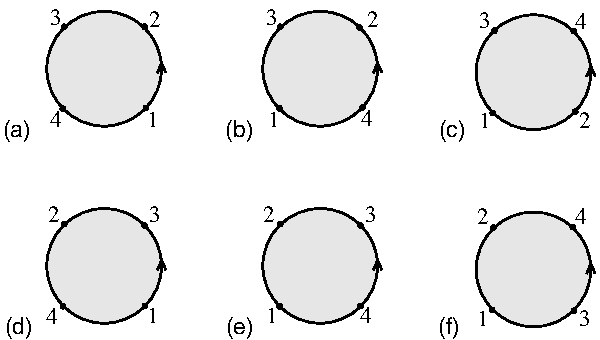
\includegraphics[width=0.9\linewidth]{figures/fig_6_2.pdf}
\caption{円板上の四つの開弦頂点演算子の、巡回的に非同値な六つの順序。座標 $y$ は矢印の向きに増加する。ただし点3では $+\infty$ から $-\infty$ へ飛ぶ。}\label{fig:6.2}
\end{figure}

これも、$y_4$ の変数変換（Möbius 変換）を行えば、$y_{1,2,3}$ に依存しない。$y_1=0$、$y_2=1$、$y_3\to\infty$ と取ると便利である。振幅は通常、Mandelstam 変数
\begin{equation}
s=-(k_1+k_2)^2,\qquad t=-(k_1+k_3)^2,\qquad u=-(k_1+k_4)^2
\tag{6.4.6}\label{eq:6.4.6}
\end{equation}
で書かれる。これらは独立ではない。運動量保存と質量殻条件から
\begin{equation}
s+t+u=\sum_i m_i^2=-\frac4{\alpha'}
\tag{6.4.7}\label{eq:6.4.7}
\end{equation}
が従う。$2\alpha'k_i\cdot k_j=-2+\alpha'(k_i+k_j)^2$ を用いると、振幅は
\begin{equation}
\begin{aligned}
S_{D_2}(k_1;k_2;k_3;k_4)&=ig_{\mathrm o}^4C_{D_2}(2\pi)^{26}\delta^{26}\!\left(\sum_i k_i\right)\\
&\quad\times\left[\int_{-\infty}^{\infty}dy_4\,|y_4|^{-\alpha'u-2}|1-y_4|^{-\alpha't-2}+(t\to s)\right]
\end{aligned}
\tag{6.4.8}\label{eq:6.4.8}
\end{equation}
となる。

積分は、$-\infty<y_4<0$、$0<y_4<1$、$1<y_4<\infty$ の三つの領域に分かれる。これら三つの領域では、頂点演算子はそれぞれ図\ref{fig:6.2}(a)、(b)、(c) のように並ぶ。Möbius 不変性を用いれば、これらの領域のどれでも他の領域へ写せるので、それらの寄与は頂点演算子の入れ替えを除いて等しい。$(t\leftrightarrow s)$ の項が図\ref{fig:6.2}(d)、(e)、(f) を与える。全部を合わせると、
\begin{equation}
\begin{aligned}
S_{D_2}(k_1;k_2;k_3;k_4)&=2ig_{\mathrm o}^4C_{D_2}(2\pi)^{26}\delta^{26}\!\left(\sum_i k_i\right)\\
&\quad\times\bigl[I(s,t)+I(t,u)+I(u,s)\bigr],
\end{aligned}
\tag{6.4.9}\label{eq:6.4.9}
\end{equation}
ただし
\begin{equation}
I(s,t)=\int_0^1dy\,y^{-\alpha's-2}(1-y)^{-\alpha't-2}.
\tag{6.4.10}\label{eq:6.4.10}
\end{equation}
三つの項は、それぞれ図\ref{fig:6.2}(c)、(f)、図\ref{fig:6.2}(b)、(d)、そして図\ref{fig:6.2}(a)、(e) から生じる。

\begin{figure}[htbp]
\centering
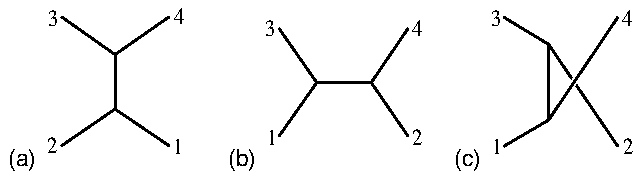
\includegraphics[width=0.9\linewidth]{figures/fig_6_3.pdf}
\caption{(a) $s$、(b) $t$、(c) $u$ チャネルの極を生じる過程。}\label{fig:6.3}
\end{figure}

積分 $I(s,t)$ は $\alpha's<-1$ かつ $\alpha't<-1$ なら収束する。$\alpha's\to-1$ では、積分は $y=0$ で発散する。この発散を調べるため、$y=0$ の近傍を取り、被積分関数を近似する：
\begin{equation}
\begin{aligned}
I(s,t)&=\int_0^rdy\,y^{-\alpha's-2}
+\text{$\alpha's=-1$ で解析的な項}\\
&=-\frac{r^{-\alpha's-1}}{\alpha's+1}
+\text{$\alpha's=-1$ で解析的な項}\\
&=-\frac1{\alpha's+1}
+\text{$\alpha's=-1$ で解析的な項}.
\end{aligned}
\tag{6.4.11}\label{eq:6.4.11}
\end{equation}
\hyperref[eq:6.4.11]{(6.4.11)} では、収束する領域で積分を評価した。この発散は、開弦タキオンの質量の二乗 $s=-1/\alpha'$ における極であることが分かる。変数 $s$ は散乱 $1+2\to3+4$ における重心系エネルギーの二乗そのものなので、この極は中間タキオン状態による共鳴である。ここでも、最も軽い弦の状態がタキオンであることはボース弦に特有であり、議論の本質には関係しない。この極は図\ref{fig:6.3}(a) に示した過程による。タキオン1と2が結合して一つのタキオンになり、これがタキオン3と4に分裂する。

$\alpha's=-1$ の特異点は単なる極なので、$I(s,t)$ はこの点を越えて $\alpha's>-1$ の領域へ解析接続できる。振幅は、この解析接続によって定義される。極における振幅の発散は、振幅の本質的な物理的特徴であり、中間の弦状態が時空の長距離を伝播することに対応する共鳴である。一方、極を越えたところで積分が発散することは、そうではない。それは振幅のこの特定の積分表示に由来するだけである。接続に問題はない。実際、弦の発散はすべて、この同じ基本的な形を持つことが分かるので、この一種類の解析接続によって、もちろん極そのものを除くすべての発散が取り除かれる。極は実軸上にあるため、さらに正確に定義する必要がある。Minkowski 過程に対する正しい $\epsilon$ 処方は
\begin{equation}
\begin{aligned}
\frac1{\alpha's+1}&\equiv\frac1{\alpha's+1+i\epsilon}\\
&\equiv\mathrm P\frac1{\alpha's+1}-i\pi\delta(\alpha's+1),
\end{aligned}
\tag{6.4.12}\label{eq:6.4.12}
\end{equation}
であり、$\mathrm P$ は主値を表す。ユニタリー性（第9章でより体系的に展開する）は、この極が存在することを要求し、その係数を、二つのタキオンが一つへ散乱する振幅によって決める：
\begin{equation}
\begin{aligned}
S_{D_2}(k_1;k_2;k_3;k_4)
&=i\int\frac{d^{26}k}{(2\pi)^{26}}
\frac{S_{D_2}(k_1;k_2;k)S_{D_2}(-k;k_3;k_4)}{-k^2+\alpha'^{-1}+i\epsilon}\\
&\quad+\text{$k^2=1/\alpha'$ で解析的な項}.
\end{aligned}
\tag{6.4.13}\label{eq:6.4.13}
\end{equation}

$I(u,s)$ からの等しい極への寄与も含めて、4タキオン振幅の因子をまとめ、3タキオンの結果 \hyperref[eq:6.4.4]{(6.4.4)} を用いると、条件 \hyperref[eq:6.4.13]{(6.4.13)} は
\begin{equation}
C_{D_2}=e^{-\lambda}C_{D_2}^XC_{D_2}^{\mathrm g}
=\frac1{\alpha'g_{\mathrm o}^2}
\tag{6.4.14}\label{eq:6.4.14}
\end{equation}
を与える。このとき3タキオン振幅は
\begin{equation}
S_{D_2}(k_1;k_2;k_3)=\frac{2ig_{\mathrm o}}{\alpha'}(2\pi)^{26}\delta^{26}\!\left(\sum_i k_i\right).
\tag{6.4.15}\label{eq:6.4.15}
\end{equation}
さまざまな汎関数行列式は消えた。ユニタリー性を用いれば、すべての規格化を、頂点演算子に現れる定数 $g_{\mathrm o}$ で表せる。実際には、行列式は注意深い正則化と繰り込みによって計算でき、異なるトポロジー間の相対的な規格化は、ユニタリー性から求めたものと一致する。

極を越えて接続すると、さらに特異点に出会う。被積分関数を $y=0$ で Taylor 展開すると、
\begin{equation}
I(s,t)=\int_0^rdy\,\left[y^{-\alpha's-2}+(\alpha't+2)y^{-\alpha's-1}+\cdots\right].
\tag{6.4.16}\label{eq:6.4.16}
\end{equation}
第2項は $\alpha's=0$ に極を与える：
\begin{equation}
I(s,t)=\frac{u-t}{2s}+\text{$\alpha's=0$ で解析的な項}.
\tag{6.4.17}\label{eq:6.4.17}
\end{equation}
Taylor 展開のさらに先の項から、振幅は
\begin{equation}
\alpha's=-1,0,1,2,\ldots
\tag{6.4.18}\label{eq:6.4.18}
\end{equation}
に極を持つ。これらは開弦の状態の位置と正確に一致する。積分 $I(s,t)$ は、変数 $t$ についても同じ位置 \hyperref[eq:6.4.18]{(6.4.18)} に極を持ち、これは端点 $y=1$ から生じる。これらは図\ref{fig:6.3}(b) の過程による。振幅 \hyperref[eq:6.4.9]{(6.4.9)} の残りの二つの項は、$s$ および $t$ チャネルの極にさらに寄与し、また図\ref{fig:6.3}(c) の $u$ チャネルの極も与える。\hyperref[eq:6.4.17]{(6.4.17)} の $s=0$ における留数は $u-t$ の奇関数なので、この極は実際には $I(s,u)$ からの極と相殺し、$1/\alpha'$ の偶数倍にあるすべての極も同様に相殺する。次節で導入する、より一般的な開弦理論では、こうはならない。

Euler のベータ関数を
\begin{equation}
B(a,b)=\int_0^1dy\,y^{a-1}(1-y)^{b-1}
\tag{6.4.19}\label{eq:6.4.19}
\end{equation}
と定義すると、
\begin{equation}
I(s,t)=B(-\alpha_{\mathrm o}(s),-\alpha_{\mathrm o}(t)),
\qquad \alpha_{\mathrm o}(x)=1+\alpha'x.
\tag{6.4.20}\label{eq:6.4.20}
\end{equation}
これはガンマ関数で表すことができる。$w$ を固定し、$y=v/w$ と置くと、
\begin{equation}
w^{a+b-1}B(a,b)=\int_0^w dv\,v^{a-1}(w-v)^{b-1}.
\tag{6.4.21}\label{eq:6.4.21}
\end{equation}
両辺に $e^{-w}$ を掛け、$\int_0^\infty dw$ で積分し、まとめ直すと、
\begin{equation}
\begin{aligned}
\Gamma(a+b)B(a,b)&=\int_0^\infty dv\,v^{a-1}e^{-v}
\int_0^\infty d(w-v)\,(w-v)^{b-1}e^{-(w-v)}\\
&=\Gamma(a)\Gamma(b).
\end{aligned}
\tag{6.4.22}\label{eq:6.4.22}
\end{equation}
したがって4タキオン振幅は
\begin{equation}
\begin{aligned}
&S_{D_2}(k_1;k_2;k_3;k_4)=\frac{2ig_{\mathrm o}^2}{\alpha'}(2\pi)^{26}\delta^{26}\!\left(\sum_i k_i\right)\\
&\quad\times\bigl[B(-\alpha_{\mathrm o}(s),-\alpha_{\mathrm o}(t))
+B(-\alpha_{\mathrm o}(s),-\alpha_{\mathrm o}(u))
+B(-\alpha_{\mathrm o}(t),-\alpha_{\mathrm o}(u))\bigr],
\end{aligned}
\tag{6.4.23}\label{eq:6.4.23}
\end{equation}
ただし
\begin{equation}
B(-\alpha_{\mathrm o}(x),-\alpha_{\mathrm o}(y))
=\frac{\Gamma(-\alpha'x-1)\Gamma(-\alpha'y-1)}{\Gamma(-\alpha'x-\alpha'y-2)}.
\tag{6.4.24}\label{eq:6.4.24}
\end{equation}
これが \emph{Veneziano 振幅}であり、もともとは強い相互作用の現象論的な特徴の一部を模型化するために書かれた。

Veneziano 振幅の高エネルギーでの振る舞いは重要である。注目すべき領域は二つあり、Regge 極限
\begin{equation}
s\to\infty,\qquad t\ \text{を固定}
\tag{6.4.25}\label{eq:6.4.25}
\end{equation}
と、硬散乱極限
\begin{equation}
s\to\infty,\qquad t/s\ \text{を固定}
\tag{6.4.26}\label{eq:6.4.26}
\end{equation}
である。散乱過程 $1+2\to3+4$ を考えると（したがって $k_1^0$ と $k_2^0$ は正であり、$k_3^0$ と $k_4^0$ は負である）、1と2の重心系では
\begin{equation}
s=E^2,\qquad t=(4m^2-E^2)\sin^2\frac\theta2,
\qquad u=(4m^2-E^2)\cos^2\frac\theta2,
\tag{6.4.27}\label{eq:6.4.27}
\end{equation}
となる。$E$ は重心系エネルギー、$\theta$ は粒子1と粒子3の間の角度である。Regge 極限は高エネルギー・小角の極限であり、硬散乱極限は高エネルギー・固定角の極限である。Stirling の近似 $\Gamma(x+1)\approx x^xe^{-x}(2\pi x)^{1/2}$ を用いると、Regge 領域での振る舞いは
\begin{equation}
S_{D_2}(k_1;k_2;k_3;k_4)\propto s^{\alpha_{\mathrm o}(t)}\Gamma(-\alpha_{\mathrm o}(t)),
\tag{6.4.28}\label{eq:6.4.28}
\end{equation}
となり、ここでも $\alpha_{\mathrm o}(t)=\alpha't+1$ である。すなわち、振幅は $s$ のべきとして変化し、そのべきは $t$ に依存する。これが Regge の振る舞いである。ガンマ関数の極では、振幅は $s$ の整数べきであり、整数スピン $\alpha_{\mathrm o}(t)$ を持つ弦の交換に対応する。

硬散乱極限では、
\begin{equation}
\begin{aligned}
S_{D_2}(k_1;k_2;k_3;k_4)
&\approx\exp\left[-\alpha'(s\ln s\alpha'+t\ln t\alpha'+u\ln u\alpha')\right]\\
&=\exp[-\alpha'sf(\theta)],
\end{aligned}
\tag{6.4.29}\label{eq:6.4.29}
\end{equation}
ただし
\begin{equation}
f(\theta)\approx-\sin^2\frac\theta2\ln\sin^2\frac\theta2
-\cos^2\frac\theta2\ln\cos^2\frac\theta2
\tag{6.4.30}\label{eq:6.4.30}
\end{equation}
は正である。結果 \hyperref[eq:6.4.29]{(6.4.29)} は注目に値する。高エネルギー・固定角の散乱は、散乱される物体の内部構造を探る。Rutherford は、アルファ粒子と原子の硬散乱によって原子核を発見した。SLAC における電子と核子の硬散乱は、核子を構成するクォークを明らかにした。場の量子論では、硬散乱振幅は $s$ のべきとして減衰する。核子のような複合物体でも、その構成要素が点状なら、振幅はべき則に従う。指数関数的な減衰 \hyperref[eq:6.4.29]{(6.4.29)} は、それよりはるかに軟らかい。結果 \hyperref[eq:6.4.29]{(6.4.29)} は、予想されるように、大きさ $\alpha'^{1/2}$ の滑らかな物体を示唆する。

ここでは0粒子、1粒子、2粒子の振幅を飛ばして、3粒子振幅から始めた。これらの振幅とその解釈は、第6.6節で議論する。

